\documentclass[border=5pt]{standalone}
\usepackage{tikz}
\usetikzlibrary{arrows.meta, positioning, decorations.pathreplacing}
\usepackage{xcolor}

\definecolor{Garnet}{HTML}{73000A}
\definecolor{NinetyBlack}{HTML}{363636}
\definecolor{SeventyBlack}{HTML}{5C5C5C}
\definecolor{FiftyBlack}{HTML}{A2A2A2}
\definecolor{ThirtyBlack}{HTML}{C7C7C7}
\definecolor{TenBlack}{HTML}{ECECEC}
\definecolor{Atlantic}{HTML}{466A9F}

\tikzset{every node/.append style={rounded corners=0pt}}

\begin{document}
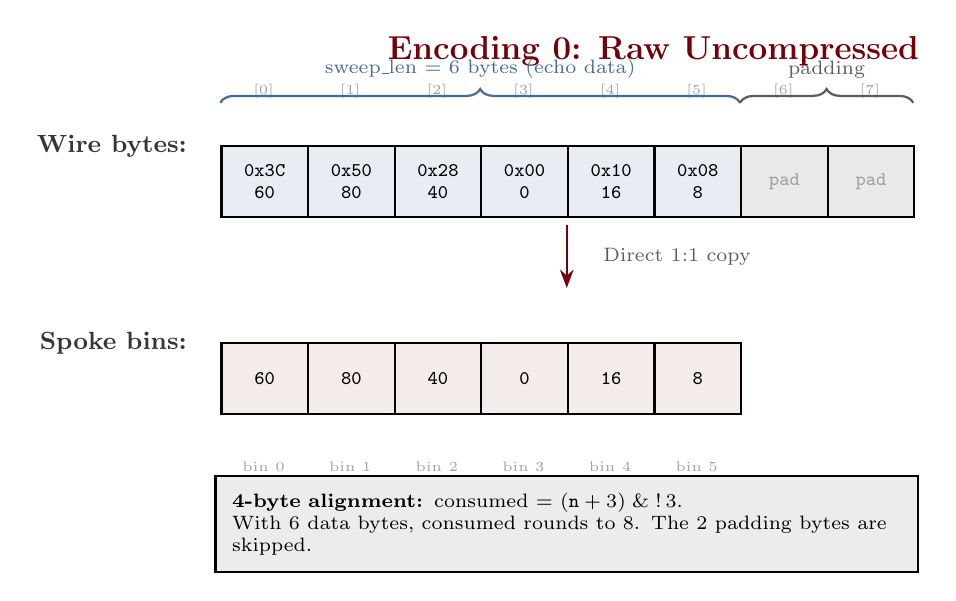
\begin{tikzpicture}[
    cell/.style={draw, thick, minimum width=1.1cm, minimum height=0.9cm, anchor=west, font=\ttfamily\scriptsize, align=center},
    lbl/.style={font=\small\bfseries, color=NinetyBlack},
    annot/.style={font=\scriptsize, color=SeventyBlack},
]

\node[font=\bfseries\large, color=Garnet] at (5.5, 3.2) {Encoding 0: Raw Uncompressed};

% Wire bytes row
\node[lbl, anchor=east] at (-0.3, 2) {Wire bytes:};
\node[cell, fill=Atlantic!12] (w0) at (0, 1.55) {\texttt{0x3C}\\60};
\node[cell, fill=Atlantic!12] (w1) at (1.1, 1.55) {\texttt{0x50}\\80};
\node[cell, fill=Atlantic!12] (w2) at (2.2, 1.55) {\texttt{0x28}\\40};
\node[cell, fill=Atlantic!12] (w3) at (3.3, 1.55) {\texttt{0x00}\\0};
\node[cell, fill=Atlantic!12] (w4) at (4.4, 1.55) {\texttt{0x10}\\16};
\node[cell, fill=Atlantic!12] (w5) at (5.5, 1.55) {\texttt{0x08}\\8};
\node[cell, fill=ThirtyBlack!40] (w6) at (6.6, 1.55) {\color{FiftyBlack}pad};
\node[cell, fill=ThirtyBlack!40] (w7) at (7.7, 1.55) {\color{FiftyBlack}pad};

% Byte indices
\foreach \i in {0,...,7} {
    \node[font=\tiny, color=FiftyBlack, above=1pt] at (0.55 + \i*1.1, 2.45) {[\i]};
}

% Brace over data
\draw[decorate, decoration={brace, amplitude=5pt}, thick, Atlantic]
    (0, 2.55) -- (6.6, 2.55) node[midway, above=5pt, font=\scriptsize, color=Atlantic] {sweep\_len = 6 bytes (echo data)};

% Brace over padding
\draw[decorate, decoration={brace, amplitude=5pt}, thick, SeventyBlack]
    (6.6, 2.55) -- (8.8, 2.55) node[midway, above=5pt, font=\scriptsize, color=SeventyBlack] {padding};

% Arrow down
\draw[-{Stealth}, thick, Garnet] (4.4, 1.0) -- (4.4, 0.2);
\node[annot] at (5.8, 0.6) {Direct 1:1 copy};

% Decoded spoke row
\node[lbl, anchor=east] at (-0.3, -0.5) {Spoke bins:};
\node[cell, fill=Garnet!8] (s0) at (0, -0.95) {60};
\node[cell, fill=Garnet!8] (s1) at (1.1, -0.95) {80};
\node[cell, fill=Garnet!8] (s2) at (2.2, -0.95) {40};
\node[cell, fill=Garnet!8] (s3) at (3.3, -0.95) {0};
\node[cell, fill=Garnet!8] (s4) at (4.4, -0.95) {16};
\node[cell, fill=Garnet!8] (s5) at (5.5, -0.95) {8};

\foreach \i in {0,...,5} {
    \node[font=\tiny, color=FiftyBlack, below=1pt] at (0.55 + \i*1.1, -1.85) {bin \i};
}

% Alignment note
\node[draw, thick, fill=TenBlack, text width=8.5cm, align=left, font=\scriptsize, inner sep=6pt] at (4.4, -2.8)
    {\textbf{4-byte alignment:} consumed = $(\texttt{n} + 3)\; \&\; !\,3$. \\
     With 6 data bytes, consumed rounds to 8. The 2 padding bytes are skipped.};

\end{tikzpicture}
\end{document}
